%!TEX root=../main.tex
\chapter{Network motifs}\label{sec:motifs}

Graphs representing networks, including biological networks and social networks, include wide variety of subgraphs. One important local property of networks are so-called \emph{network motifs}, which are defined as recurrent and statistically significant sub-graphs or patterns.

Network motifs are sub-graphs that repeat themselves in a specific network or even among various networks. Each of these sub-graphs, defined by a particular pattern of interactions between vertices, may reflect a framework in which particular functions are achieved efficiently. Indeed, motifs are of notable importance largely because they may reflect functional properties.

Let's start by the simplest network motifs, the triangles.

\section{Triangles}
The triangle is, unsurprisingly, defined as a triple of nodes for which each of the three pairs of node is connected. 
We would like to compute the \emph{global clustering coefficient}.
\[
	c(G) = \frac{3 \cdot \left(\text{\# triangles in G}\right)}{\left(\text{\# connected triples in G}\right)} = \frac{3 \mathcal{T}}{w(G)}
\]
%
Let's compute this on an example.
%
\begin{figure}[h!]
	\centering
	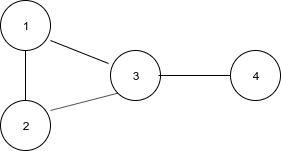
\includegraphics[width=.4\textwidth]{graph-triangle-example.png}
	\caption{Graph example}\label{fig:graph-example-triangles}
\end{figure}

In the graph shown in \cref{fig:graph-example-triangles} there are $5$ connected triples and $1$ triangle, so the global clustering coefficient would be $3/5$.
%
\begin{figure}[h!]
	\centering
	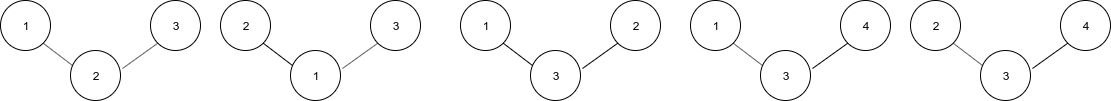
\includegraphics[width=\textwidth]{conn-triples.png}
\end{figure}

The \emph{g.c.c.} for a clique is $1$, because every connected triple is also a triangle; while for a star it is $0$ because there are no triangles.

To compute the denominator for the \emph{g.c.c.}, that is $w(g)$, what we can do is sum all the pairs of nodes in the neighborhood of each node.
\[
	w(G) = \sum_{u \in V}\binom{d(u)}{2}
\]
taking $T = O(N)$.
This gives us a first algorithm to compute the \emph{g.c.c.}
%
\begin{lstlisting}[caption={Algorithm 1}, label={alg:triangles-alg1}]
Algorithm_1:
    for $u \in V$
        for $\{ v, w \} \in \binom{N_u}{2}$:
            if $\{ v, w \} \in E$:
                $\mathcal{T} += 1$
    return $\frac{\mathcal{T}}{3}$
\end{lstlisting}
%
\begin{claim}
	Algorithm is in $O(n^3)$.
\end{claim}
\begin{proof}
	If the graph is dense, that is the degree for each node $u$ is close to $n^2$, we have that:
	\[
		\sum_{u \in V}\binom{d_u}{2} = \sum_{u \in V}\Omega(n^2) = \Omega(n^3)
	\]
	while if the $max-degree$ is constant, we have that:
	\[
		\sum_{u \in V}\binom{d_u}{2} = \sum_{u \in V} const = O(n)
	\]
\end{proof}

\section{Adjacency Matrix method}

One algorithm to compute the number of triangles is based on the adjacency matrix multiplication.
The adjacency matrix for the graph seen in \cref{fig:graph-example-triangles} is the following
\[
	\begin{pmatrix}
		0 & 1 & 1 & 0 \\
		1 & 0 & 1 & 0 \\
		1 & 1 & 0 & 1 \\
		0 & 0 & 1 & 0 \\
	\end{pmatrix}
\]
Let's compute the square of it.
\[
	A^2 = 	\begin{pmatrix}
		2 & 1 & 1 & 1 \\
		1 & 2 & 1 & 1 \\
		1 & 1 & 3 & 0 \\
		1 & 1 & 0 & 1 \\
	\end{pmatrix}
\]
Now, what does the $ij$ cell contain? by definition of matrix multiplication we have that
\[
	(A^2)_{ij} = \sum_{w \in G}A_{uw} \cdot A_{wv}
\]
where $A_{uw} = 1$ iff $(u,w) \in E$ and  $A_{wv} = 1$ iff $(w,v) \in E$. In other words, we are counting the number of paths of length $2$ that go from $u$ to $w$.
In cell $A_{uu}$ there is the number of paths of length $2$ that go from $u$ to itself, that is equal to its degree because we can go from $u$ to any of its neighbours in $1$ step and then use the same edge to go back to $u$.
Intuitively, $(A^3)_{uv}$ contains the number of paths of length $3$ that go from $u$ to $v$, and in general the same reasoning applies to any $A^k$ for paths of length $k$.

To find triangles we can compute $A^3$ and, for every node, get its diagonal entry in the matrix, effectively giving us the number of paths of length $3$ that go from that node to itself.
%
\begin{figure}[h!]
	\centering
	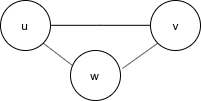
\includegraphics[width=.5\textwidth]{triangle.png}
	\caption{A triangle.}\label{fig:triangle-graph}
\end{figure}
% 
Let's compute $(A^3)_{uu}$ in \cref{fig:triangle-graph}; there are two paths of length $3$ that go from $u$ to itself: $uvw, uwv$. So $(A^3)_{uu}$ would be $2$, but the node is in just one triangle.
That is true in general, so every triangle gives a contribute of $2$ to the diagonal entry of every node that forms it. Furthermore, this way we will count the same triangle $3$ times. We thus have
\[
	\sum_{u \in G}{\left(A^3\right)_{uu}} = tr(A^3) = 6 \cdot \mathcal{T}(G)
\]
\begin{thm}
	$$\mathcal{T}(G) = \frac{tr(A^3)}{6}$$
\end{thm}

This gives us the following algorithm:
\begin{lstlisting}[caption={Algorithm 2}, label={alg:triangles-alg2}]
Algorithm_2(A: AdjacencyMatrix):
    $AC \gets$ fast_mat_multiplication(A,3)
    return $\frac{tr(AC)}{6}$
\end{lstlisting}